\makeatletter
\def\input@path{{../../}}
\makeatother
\documentclass[../../main.tex]{subfiles}

\graphicspath{
	{../../img/}
	{../img/}
	{img/}
}

\begin{document}
\section{Поточечная и равномерная сходимость рядов и последовательностей ФКП}

Рассмотрим последовательность $ \phi_n,\, n \in \N $ ФКП, определенную для $ z \in D $ ~--- односвязной области.

$ \phi_n(z) $ сходится поточечно к $ f(z), z \in D $, если

\begin{equation}\label{34:1}
	\forall\, \varepsilon > 0 \quad \forall\, z \in D \quad \exists\, \nu = \nu_\varepsilon (z) \in \R\, :\, \forall\, n \geq \nu \implies |\phi_n(z) - f(z)| \leq \varepsilon
\end{equation}

\[ \implies \exists\, \underset{n \to \infty}{\lim} \phi_n (z) = f(z),\, \forall z \in D \quad \phi_n(z) \overset{D}{\underset{n \to \infty}\longrightarrow} f(z) \]

Последовательность $ (\phi_n(z)) $ называется равномерно сходящейся к $ f(z) $, если

\begin{equation}\label{34:2}
	\forall\, \varepsilon > 0 \quad \exists\, \nu = \nu_\varepsilon (z) \in \R\, :\, \forall\, n \geq \nu,\, \forall z \in D \implies |\phi_n(z) - f(z)| \leq \varepsilon
\end{equation}

$ \eqref{34:2} $ записывают следующим образом

\[ \phi_n(z) \overset{D}{\underset{n \to \infty}\rightrightarrows} f(z) \]

Нетрудно видеть, что из $ \eqref{34:2} \implies \eqref{34:1} $. Обратное, вообще говоря, неверно.

Здесь, как и в $\R$ случае, справедливы следующие теоремы.

\begin{thm}{Супремальный критерий равномерной сходимости ФПКП}
	\[ \phi_n(z) \overset{D}{\underset{n \to \infty}\rightrightarrows} f(z) \iff \underset{x \in E}{\sup}|\phi_n(z) - f(z)| \appr{n \rightarrow \infty} 0 \]
\end{thm}

\begin{thm}{Мажорантный признак равномерной сходимости ФПКП.}
	\;
	
	Если 
	\[ \exists\, a_n \geq 0 \in \R :\, |\phi_n(z) - f(z)| \leq a_n,\, \forall n \in \N,\, \forall z \in D, \]
	и если \[ a_n \appr{n \rightarrow \infty} \infty, \]
	то \[ \phi_n(z) \overset{D}{\underset{n \to \infty}\rightrightarrows} f(z) \]
\end{thm}

\begin{thm}{Достаточное условие неравномерной сходимости}
	\;
	
	Если
	\[ \exists (z_n) \in D\, :\, |\phi_n(z_n) - f(z_n)| \underset{n \to \infty}{\not \rightarrow} 0, \]
	то
	\[ \phi_n(z) \overset{D}{\underset{n \to \infty}{\not \rightrightarrows}} f(z) \]
\end{thm}

Обобщаются также следующие результаты равномерной сходимости действительных ФП на комплексные ФП: теорема Стокса-Зейделя, предельный переход, дифференцирование и интегрирование.

Для ФР $ \sum\limits_{n = 1}^{\infty} u_n(z) = u_1(z) + \ldots + u_n(z), z \in D $ поточечная и равномерная сходимость определяется через соответствующую сходимость последовательности частных сумм $ S_n(z) = \sum\limits_{k = 1}^{n} u_k(z): $

\begin{enumerate}
	\item $ \sum\limits_{n = 1}^{\infty} u_n(z) \overset{D}{\longrightarrow} S(z) \iff S_n(z) \overset{D}{\underset{n \to \infty}\longrightarrow} S(z) $
	
	\item $ \sum\limits_{n = 1}^{\infty} u_n(z) \overset{D}\rightrightarrows S(z) \iff S_n(z) \overset{D}{\underset{n \to \infty}\rightrightarrows} S(z) $
\end{enumerate}

Здесь также справедлива следующая теорема.

\begin{thm}{Мажорантный признак Вейерштрасса для ФРКП}
	\;
	
	Если
	
	\[ \exists\, a_n \geq 0\, :\, |u_n(z)| \leq a_n\, \forall\, n \in \N \quad \forall z \in D, \]
	
	то в случае, когда $ \sum\limits_{n = 1}^{\infty} a_n $ сходится, ряд $ \sum\limits_{n = 1}^{\infty} u_n(z) \overset{D}\rightrightarrows $.
\end{thm}

По аналогии со случаем $\R$ доказывается теорема Стокса-Зейделя непрерывности суммы ФРКП.

\begin{thm}{О почленном интегрировании и дифференцировании ФРКП}
	\begin{enumerate}
		\item Если $ \forall\, u_n (z) $ непрерывна на $ D $ и $ \sum\limits_{n = 1}^{\infty} u_n(z) \overset{D}\rightrightarrows f(z) $, то тогда $ f(z) $ непрерывна на $ D $.
		
		\item Если $ \forall\, u_n (z) $ непрерывна на $ D $ и $ \sum\limits_{n = 1}^{\infty} u_n(z) \overset{D}\rightrightarrows f(z) $, то для любого кусочно-гладкого контура $ l \in D $ выполнено
		
		\[ \int\limits_l \sum\limits_{n = 1}^{\infty} u_n(z) dz = \sum\limits_{n = 1}^{\infty} \int\limits_l  u_n(z) dz \]
		
		\item Если $ \forall\, u_n(z) $ непрерывно диференцируема на $ D $, и если $ \sum\limits_{n = 1}^{\infty} u_n(z) \overset{D}{\longrightarrow},\, \sum\limits_{n = 1}^{\infty} u_n^{'}(z) \overset{D}\rightrightarrows $, то $ (\sum\limits_{n = 1}^{\infty} u_n(z))' = \sum\limits_{n = 1}^{\infty} u_n^{'}(z) $
	\end{enumerate}
\end{thm}

Кроме указанных свойств равномерно сходящихся ФП и ФР КП, аналогично свойствам действительных ФП и ФР, нам понадобятся теоремы 1 и 2 Вейерштрасса для ФР КП.

\begin{thm}{1-я теорема Вейерштрасса}
	\;
	
	Пусть $ \forall\, u_n(z) $ аналитична в односвязной области $ D $. Если ряд $ \sum\limits_{n = 1}^{\infty} u_n(z) $ сходится локально равномерно в $ D $, т.е. для любого $ D_0 \subset D, D_0 $ ~--- компакт, $ \sum\limits_{n = 1}^{\infty} u_n(z) $ сходится равномерно на $ D_0 $, то тогда
	
	\begin{enumerate}
		\item  $ f(z) = \sum\limits_{n = 1}^{\infty} u_n(z) $ ~--- аналитична в $ D $.
		
		\item Рассматриваемый ФРКП можно почленно бесконечно раз дифференцировать в $ D $, т.е.
		
		\begin{equation}\label{34:3}
			 \exists\, f^{(m)}(z) = (\sum\limits_{n = 1}^{\infty} u_n(z))^{(m)} = \sum\limits_{n = 1}^{\infty} u_n^{(m)} (z), \quad \forall\, m \in \N_0,\, \forall z \in D
		\end{equation}
		
		Полученные ФР $ \eqref{34:3} $ будут локально равномерно сходится в $ D $.
	\end{enumerate}
\end{thm}

\begin{thm}{2-я теорема Вейерштрасса}
	\;
	
	Пусть $ \forall\, u_n(z) $ аналитична в области $ D $ с кусочно-гладкой границей $ l $. Если любая $ u_n(z) $ непрерывна на $ \overline{D} \in D \cup l $ и ряд $ \sum\limits_{n = 1}^{\infty} u_n(z) \overset{l}\rightrightarrows,\, $ то ряд $ \sum\limits_{n = 1}^{\infty} \overset{\overline{D}}\rightrightarrows $.
\end{thm}

\begin{proof}
	Из критерия Коши сходимости рядов ФКП следует
	
	$ \sum\limits_{n = 1}^{\infty} u_n(z) \overset{l}\rightrightarrows \iff \forall\, \varepsilon > 0\, \exists\, \nu = \nu_\varepsilon \in \R : \forall\, n, m \geq \nu $ и $ \forall\, t \in l : |S_n(t) - S_m(t)| \leq \varepsilon $
	
	Используя принцип максимума модуля, получаем, что на $ \overline{D}\, \exists\, \underset{z \in D}{max}|S_n(z) - S_m(z)| = |S_n(t_0) - S_m(t_0)| $, где $ t_0 \in l = \partial D $.
	
	Поэтому $ \forall\, \varepsilon > 0\, \exists\, \nu = \nu_\varepsilon \in \R :\, \forall\, n, m \geq \nu \cup \forall\, z \in \overline{D} \implies |S_n(z) - S_m(z)| \leq \underset{z \in D}{max}|S_n(z) - S_m(z)| \overset{\exists\, t_0 \in L}= |S_n(t_0) - S_m(t_0)| \leq \varepsilon $ 
	
	Отсюда по критерию Коши для ФР КП следует, что ряд $ \sum\limits_{n = 1}^{\infty} \overset{\overline{D}}\rightrightarrows $
\end{proof}

\section{Степенные ряды ФКП. Голоморфные ФКП}

Степенным рядом в комплексной последовательности будем называть ряд вида

\begin{equation}\label{34:4}
	\sum\limits_{n = 1}^{\infty} c_n\, (z - z_0)^n
\end{equation}

Здесь $ c_n \in \C,\, \forall\, n \in \N_0,\, z_0 \in \C $ ~--- центр степенного ряда. По той де схеме, что и для степенныз рядов в $ \R $, доказывается следующая теорема:

\begin{thm}{теорема Абеля для комплексный Степенных рядов (СтР)}
	Если $ \eqref{34:4} $ сходится в точке $ z_1 \neq z_0 $, то он будет сходится $ \forall z \in \C $, который удовлетворяет неравенству:
	
	\[ |z - z_0| < |z_1 - z_0| \]
\end{thm}

Отсюда, в частности, получаем, что существует такое $ R \geq 0, R \in \R $, что степенной ряд сходится, если $ |z - z_0| < R $ и расходится, если $ |z - z_0| > R $.

Чтобы получить полное множество сходящихся СтР, его нужно исследовать на $ |z - z_0| = R $. Здесь обычно используют параметр окрестности $ z = z_0 + e^{ir},\, 0 \leq t \leq 2\pi $ и после подстановки в $ \eqref{34:4} $ получают соответственные тригонометрические ряды, для исследования на сходимость которых можно использовать теорию рядов Фурье.

Если у ряда $ \eqref{34:4} $ все коэффициенты $ c_n $, начиная с некоторго номера, не равны нулю, то тогда, как и в $ \R $, для $R$ можно использовать либо формулу

\begin{equation}\label{34:5}
	R = \underset{n \to \infty}{\lim} |\frac{c_n}{c_{n+1}}|
\end{equation}

либо

\begin{equation}\label{34:6}
	R = \frac{1}{\underset{n \to \infty}{\lim} \sqrt[n]{|c_n|}}
\end{equation}

Если в $ \eqref{34:5} $ и $ \eqref{34:6} $ пределы не существуют, всегда можно найти $R$ по формуле Коши-Адамара

\begin{equation}\label{34:7}
	R = \frac{1}{\overline{\underset{n \to \infty}{\lim}} \sqrt[n]{|c_n|}}
\end{equation}

Круг сходимости: $ (|z - z_0| < R) $. Так как в $ \eqref{34:4} $ функции $ u_n(z) = c_n(z - z_0)^n,\, n \in \N_0) $ аналитичны всюду в $ \C $б то из 1-й теоремы Вейерштрасса следует, что сумма

\begin{equation}\label{34:8}
	f(z) = \sum\limits_{n = 0}^{\infty} c_n(z - z_0)^n
\end{equation}

будет аналитической внутри круга сходимости.

Каждую аналитическую функцию $ f(z) $, представимую в виде $ \eqref{34:8} $ в окрестности $z_0$ называют голоморфной функцией в круге сходимости.

Таким образом любая голоморфная функция в круге сходимости будет аналитической.

Тогда $ \eqref{34:8} $ можно дифференцировать почленно любое количество раз. В результате для $ \forall\, k \in \N_0 $ получим

\[ \exists\, f^{(k)}(z) = k!c_k + \frac{(k + 1!)}{1!}c_{k + 1}(z - z_0) + \ldots \]

При $ z = z_0 $ имеем

\begin{equation}\label{34:9}
	f^{(k)}(z_0) = k!c_k \implies c_k = \frac{f^{(k)}(z_0)}{k!},\, k \in \N_0
\end{equation}

В результате имеем представление

\begin{equation}\label{34:10}
	f(z) = \sum\limits_{k = 0}^{\infty} \frac{f^{(k)}(z_0)}{k!}(z - z_0)^k
\end{equation}

В общем случае, ФР $ \eqref{34:10} $ для голоморфной $ f(z) $ в круге сходимости ~--- ряд Тейлора $ f(z) $ в этом круге с центром в $ z_0 $.

Из единственного нахождения коэфициентов из $ \eqref{34:8} $ имеем единственное ее представление $ \eqref{34:10} $, и тем самым единственное разложение голоморфной функции в соответствующий степенной ряд Тейлора.

\begin{thm}{О разложении ФКП в степенной ряд}
	\;
	
	Пусть $ f(z) $ аналитична в односвязной области $ D $. Для $ fix\, z_0 \in D $ рассмотрим $ R = \underset{z \in \partial D = l}{min}d(z, z_0) $.
	
	Тогда $ f(z) $ разлагается в СтР $ \eqref{34:4} $ внутри круга $ K_R = \{z \in D | \quad |z - z_0| < R \} $, причем коэфициенты этого разложения можно вычислить по формулам $ \eqref{34:9} $.
	
	В результате получим ряд Тейлора $ \eqref{34:10} $ для $f(z)$.
\end{thm}

\begin{proof}
	Пусть $ l_R = \partial K_R = \{t \in D | \quad |t - z_0| = R \} $. Тогда для $ \forall\, z \in K_R $ и $ \forall\, t \in l_R $ имеем:
	
	\[ |z - z_0| < |t - z_0| = R, \]
	
	поэтому для \[ q = \frac{z - z_0}{t - z_0} \implies |q | = |\frac{z - z_0}{t - z_0}| < 1 \]
	
	Тогда
	
	\[ \frac{1}{t - z} = \frac{1}{(t - z_0)(1 - \frac{z - t}{t - z_0})} \leq \left[ \sum\limits_{n = 0}^{\infty}q^k = \frac{1}{1 - q}, q = \frac{z - z_0}{t - z_0} \right] = \sum\limits_{n = 0}^{\infty}\frac{(z - z_0)^n}{(t - z_0)^{n + 1}} \]
	
	Здесь, учитывая, что ряд
	
	\[ \sum\limits_{n = 0}^{\infty}\frac{(z - z_0)^n f(t)}{(t - z_0)^{n + 1}} \]
	
	сходится равноерно на $ l_R $, то его можно почленно интегрировать.
	
	\[ \frac{1}{2 \pi i} \underset{l_R}\oint \frac{f(t)}{t - r} dt\, =\, \frac{1}{2 \pi i} \sum\limits_{n = 0}^{\infty} \left( \underset{l_R}\oint\frac{f(t)dt}{(t - z_0)^{n + 1}} \right)(z - z_0)^n\, =\, \sum\limits_{n = 0}^{\infty} c_n (z - z_0)^n, \]
	
	\[ c_n = \frac{1}{2 \pi i} \underset{l_R}\oint\frac{f(t)dt}{(t - z_0)^{n + 1}} = \frac{f^{(n)}(z_0)}{n!} \]
	
	В силу интергральной формулы Коши получаем
	
	\[ f(z) = \sum\limits_{n = 0}^{\infty} \frac{f^{(n)}(z_0)}{n!} (z - z_0)^n \]
	
	Получили разложение вида $ \eqref{34:10} $ в степенной ряд, являющийся рядом Тейлора.
 \end{proof}

\begin{rem}
	\begin{enumerate}
		\item Из доказательства следует, что если $ f(z) $ разлогается в степенной ряд $ \eqref{34:4} $, то радиус сходимости $ R_{\overline{D}} $ ~--- это расстояние от $ z $ до ближайшей особой точки $ f(z) $.
		
		\item Доказанная теорема показывает, что в соответствующей окрестности $ z_0 $ понятие аналитической и голоморфной функции $f(z)$ совпадают.
		
		\item Как и в $R$, имеем следующие основные разложения в СтР:
		
		\begin{enumerate}
			\item \[ (1 + z)^\alpha = e^{ln(1 + z)} = 1 + \sum\limits_{n = 1}^{\infty} \frac{\alpha(\alpha - 1) \ldots (\alpha - n +1)}{n!}z^n,\, |z| > 1 \]
			
			\item \[ e^z = \sum\limits_{n = 0}^{\infty} \frac{z^n}{n!},\, z \in \C \]
			
			\item \[ ln(1 + z) = \sum\limits_{n = 1}^{\infty} \frac{(-1)^nz^n}{n},\, |z| \leq 1,\, z \neq -1 \]
			
			\item \[ \cos{z} = \sum\limits_{n = 0}^{\infty} \frac{(-1)^nz^{2n}}{(2n)!},\, z \in \C \]
			
			\item \[ \sin{z} = \sum\limits_{n = 0}^{\infty} \frac{(-1)^nz^{2n + 1}}{(2n + 1)!},\, z \in \C \]
			
			\item \[ \ch{z} = \sum\limits_{n = 0}^{\infty} \frac{z^{2n}}{(2n)!},\, z \in \C \]
			
			\item \[ \sh{z} = \sum\limits_{n = 0}^{\infty} \frac{z^{2n + 1}}{(2n + 1)!},\, z \in \C \]
		\end{enumerate}
	\end{enumerate}
\end{rem}

Отметим также часто возникающие на практике следующие случаи:

\begin{enumerate}
	\item \[ \frac{1}{1 - z} = \sum\limits_{n = 0}^{\infty} z^n,\, |z| < 1 \]
	
	\item \[ \frac{1}{1 + z} = \sum\limits_{n = 0}^{\infty} (-1)^nz^n,\, |z| < 1 \]

	\item \[ \frac{1}{(1 - z)^2} = \sum\limits_{n = 0}^{\infty} (n + 1)z^n,\, |z| < 1 \]
	
	\item \[ \frac{1}{(1 + z)^2} = \sum\limits_{n = 0}^{\infty} (-1)^n(n + 1)z^n,\, |z| < 1 \]
\end{enumerate}

\section{Ряд Лорана ФКП}

Рядом Лорана с центром в $ z_0 $ называется ряд вида

\begin{equation}\label{34:11}
	\sum\limits_{n = -\infty}^{\infty}c_n(z - z_0)^n = \ldots + \frac{c_{-2}}{z - z_0} + \frac{c_{-1}}{z - z_0} + c_0 + c_1(z - z_0) + c_2(z - z_0)^2 + \ldots
\end{equation}

Ряд $ \eqref{34:11} $ считается сходящимся, если одновременно сходятся ряды 

\[ \sum\limits_{n = 0}^{\infty} c_n(z - z_0)^n, \quad \text{и} \quad \sum\limits_{k = 1}^{\infty} c_{-k}t^k, \quad t = \frac{1}{z - z_0} \]

Каждый из рядов является соответствующим степенным рядом по отношению к своей переменной.

Если для первого ряда вычисляется $ R = \frac{1}{\overline{\underset{n \to \infty}{\lim}} \sqrt[n]{|c_n|}} $, то тогда ряд будет сходится, если $ |z - z_0| < R $.

Аналогично, если для второго ряда вычислить $ r_0 = \frac{1}{\overline{\underset{n \to \infty}{\lim}} \sqrt[n]{|c_n|}} $, то ряд будет сходится, если $ |z| < r_0 $, т.е. $ \frac{1}{|z - z_0|} < r_0 \implies |z - z_0| > \frac{1}{r_0} = r $, где $ r = \overline{\underset{n \to \infty}{\lim}} \sqrt[n]{|c_n|} $.

В результате получаем, что ряд Лорана $ \eqref{34:11} $ сходится, если

\[ r < |z - z_0| < R \]

В общем случаем ~--- это кольцо сходимости.

В случае, когда $ r \geq R $, кольцо сходимости будет $ \varnothing $.

Если $r = 0$, то $ 0 < |z - z_0| < R $ ~--- круг с выколотым центром $z_0$.

Если $ R = +\infty $, то кольцо сходимости дает внешность круга, соответствующего окрестности бесконечно удаленной точки.

\begin{thm}{О разложении ФКП в ряд Лорана}
	Пусть $ f(z) $ аналитична внутри некоторого кольца $ r < |z - z_0| < R,\, r \neq \varnothing $. Тогда $ f(z) $ разлогается в соответствующий ряд Лорана $ \eqref{34:11} $ и при этом коэффициенты этого разложения можно вычислить по формуле
	
	\begin{equation}\label{34:12}
		c_n = \frac{1}{2 \pi i} \underset{l_R}\oint\frac{f(t)}{(t - z_0)^{n + 1}} dt,\, n \in \Z,
	\end{equation}
	
	где $ l $ ~--- произвольный замкнутый кусочно-гладкий контур в кольце. При этом разложение в ряд Лорана единственно.
\end{thm}

\begin{proof}
	Доказательство проводится по той же схеме, что и для степенных рядов в $\Z$.
\end{proof}

\begin{exmp}
	\begin{enumerate}
		\item \[ f(z) = \frac{z + 1}{z^2 - 2z - 3} \]
		
		Особые точки функции: $ z^2 - 2z - 3 = 0, \quad z_1 = 3, z_2 = 1 $.
		
		Считая $ z_0 = 0 $ в результате плоскость $z$ разобьется на 3 области с особыми точками на границах.
		
		\begin{center}
			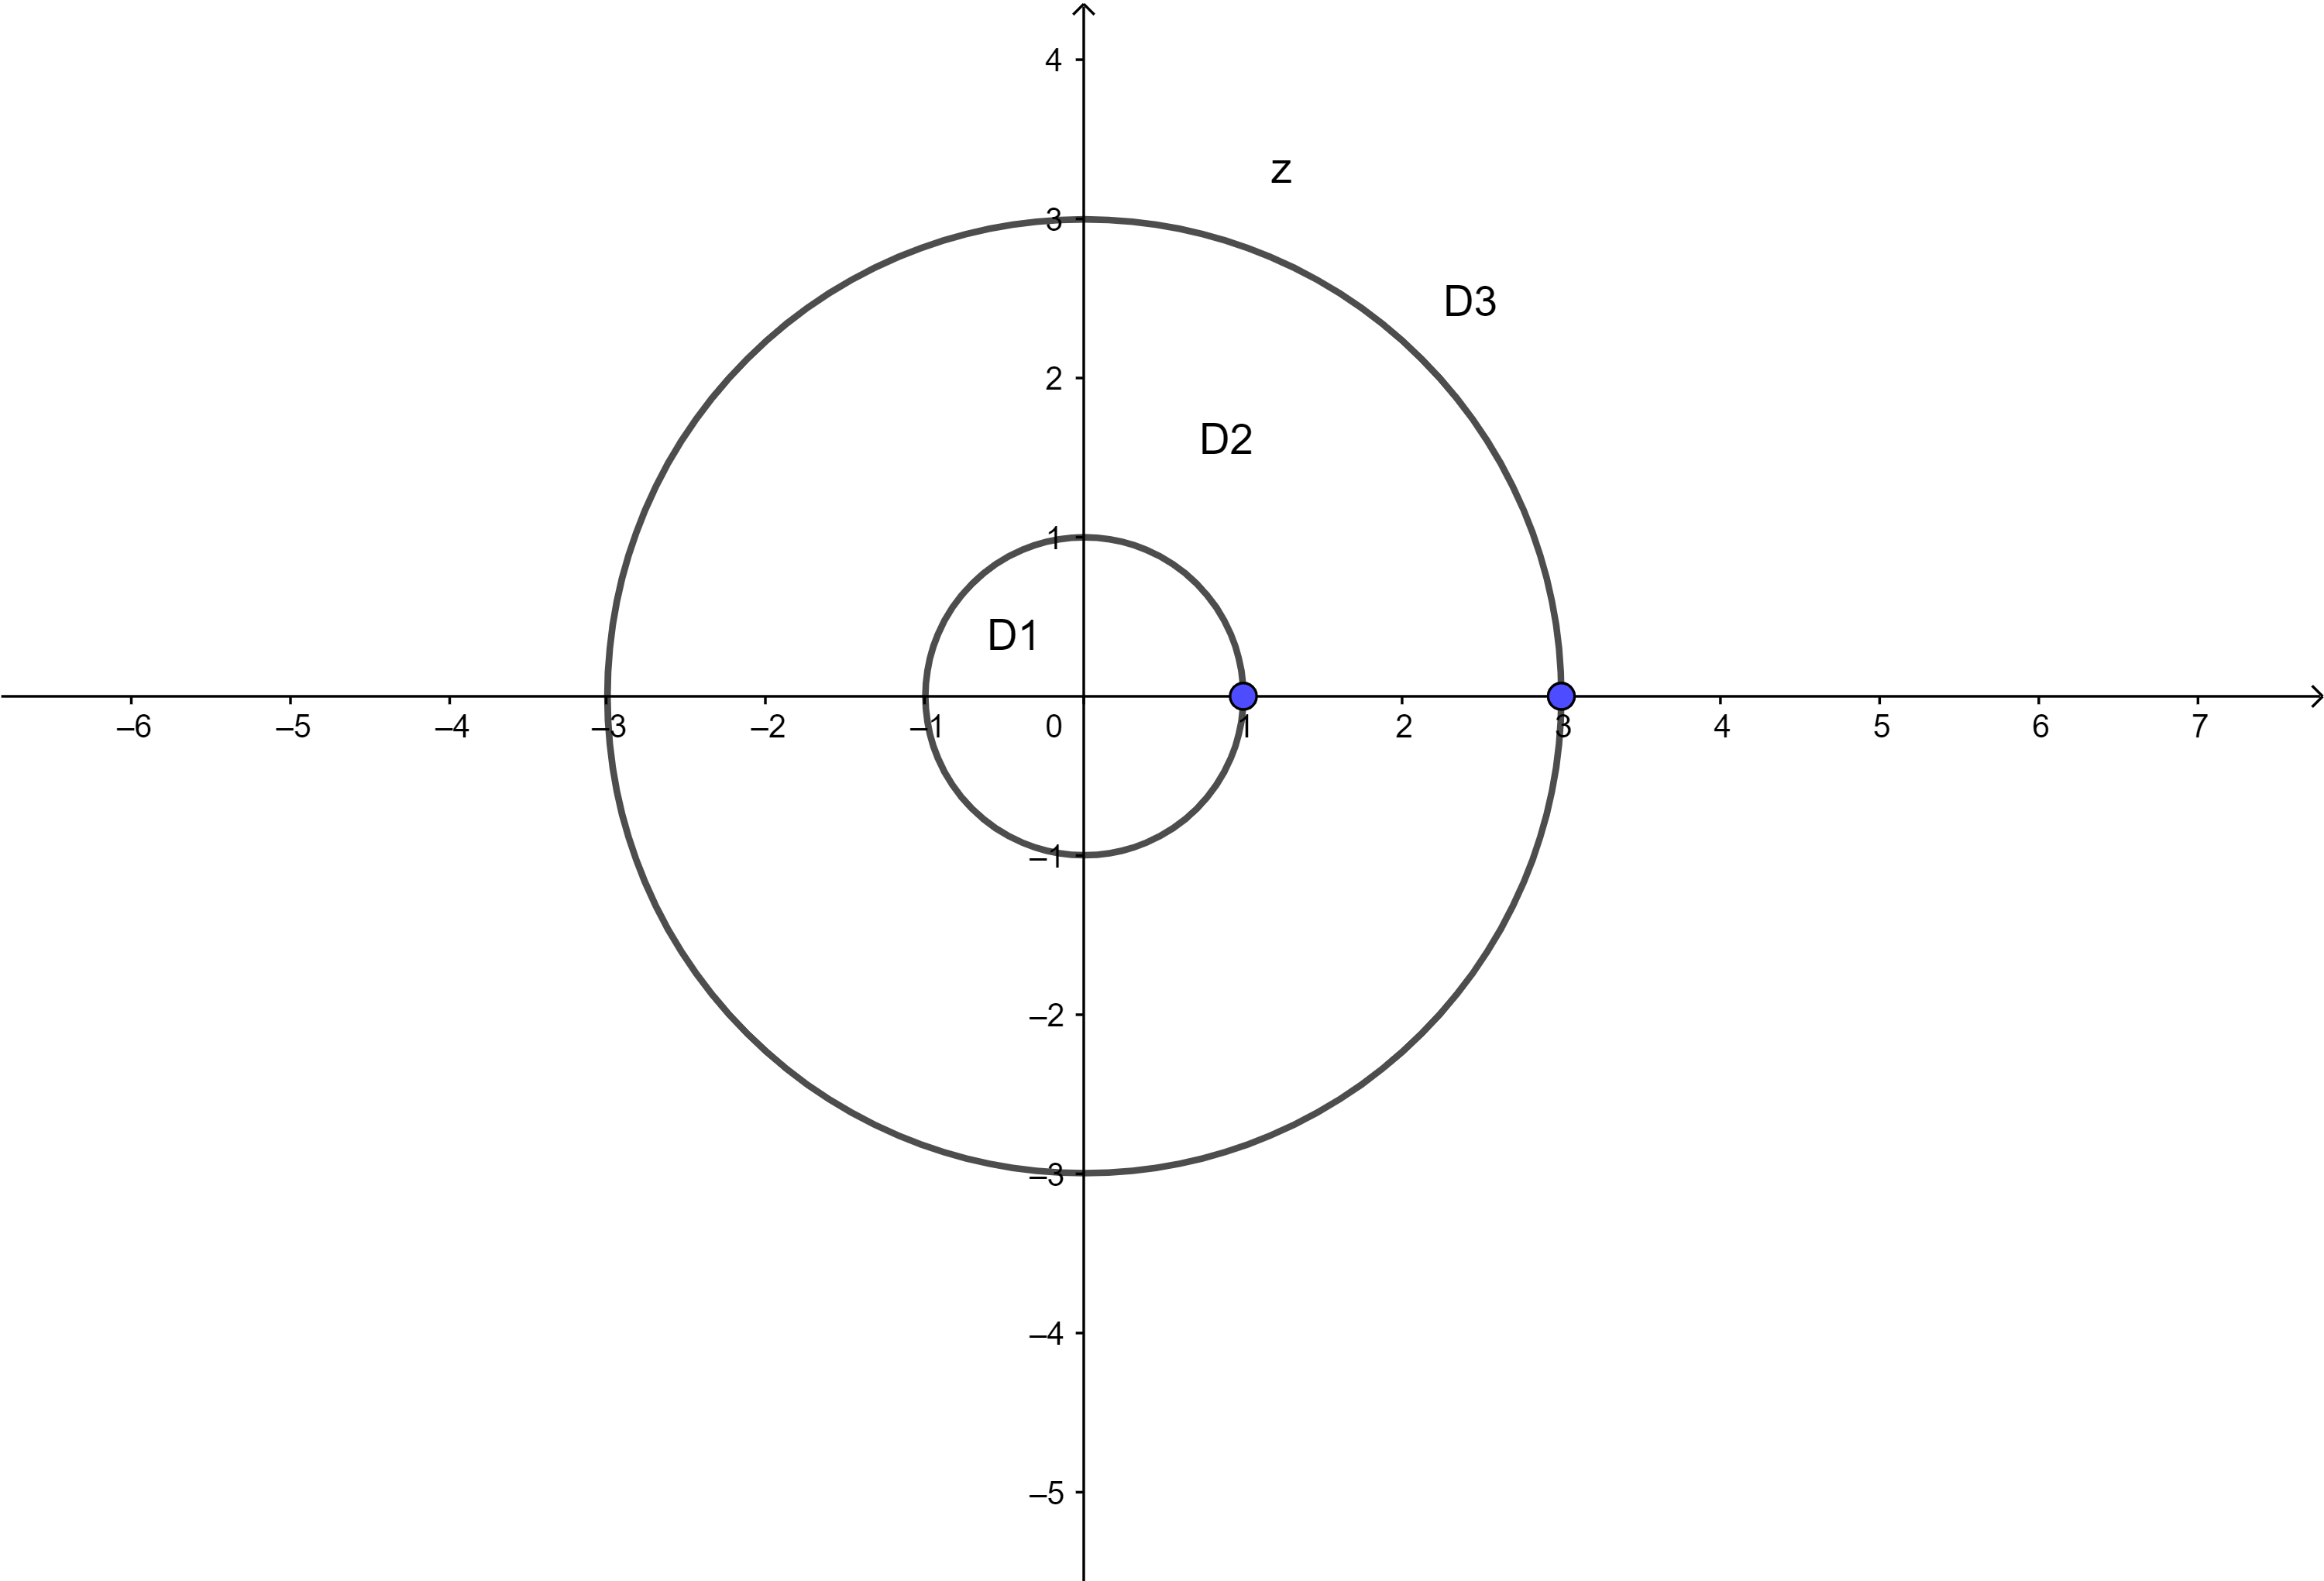
\includegraphics[scale = 0.65]{lec34_1} 
		\end{center}
		
		\begin{enumerate}
			\item В $ D_1 f(z) $ аналитична, поэтому здесь ряд Лорана дает соответствующий СтР относительно $ z > 0 $.
			
			\[ f(z) = \frac{z + 1}{(z + 1)(z - 3)} = \frac{1}{z - 3} = -\frac{\frac{1}{3}}{1 - \frac{z}{3}} = \left[ z \in D_1 \implies |z| < 1 \implies q = \frac{z}{3},\, |q| < 1 \right] = \]
			
			\[ = -\frac{1}{3} \sum\limits_{n = 0}^{\infty} \frac{z^n}{3^n} \]
			
			\item $ z \in D_2 $. Здесь будет та же логика, что и в a), так как $ -1 $ ~--- устранимая особая точка.
			
			\item $ z \in D_3 $. Здесь будет отличие только в степени $z$:
			
			\[ f(z) = \frac{1}{z(1 - \frac{3}{z})} = \left[ |z| > 3,\, |q| = |\frac{3}{z}| < 1 \right] = \frac{1}{z} \sum\limits_{n = 0}^{\infty} \frac{3^n}{z^n} = \sum\limits_{n = 0}^{\infty} \frac{3^n}{z^{n + 1}} \]
		\end{enumerate}
	
		\item \[ f(z) = \frac{1}{(z + 1)(z - 2)},\, \text{ в }\, 1 < |z| < 2 \]
		
		В этом случае получаем только одну область $ D_1 $.
		
		\begin{center}
			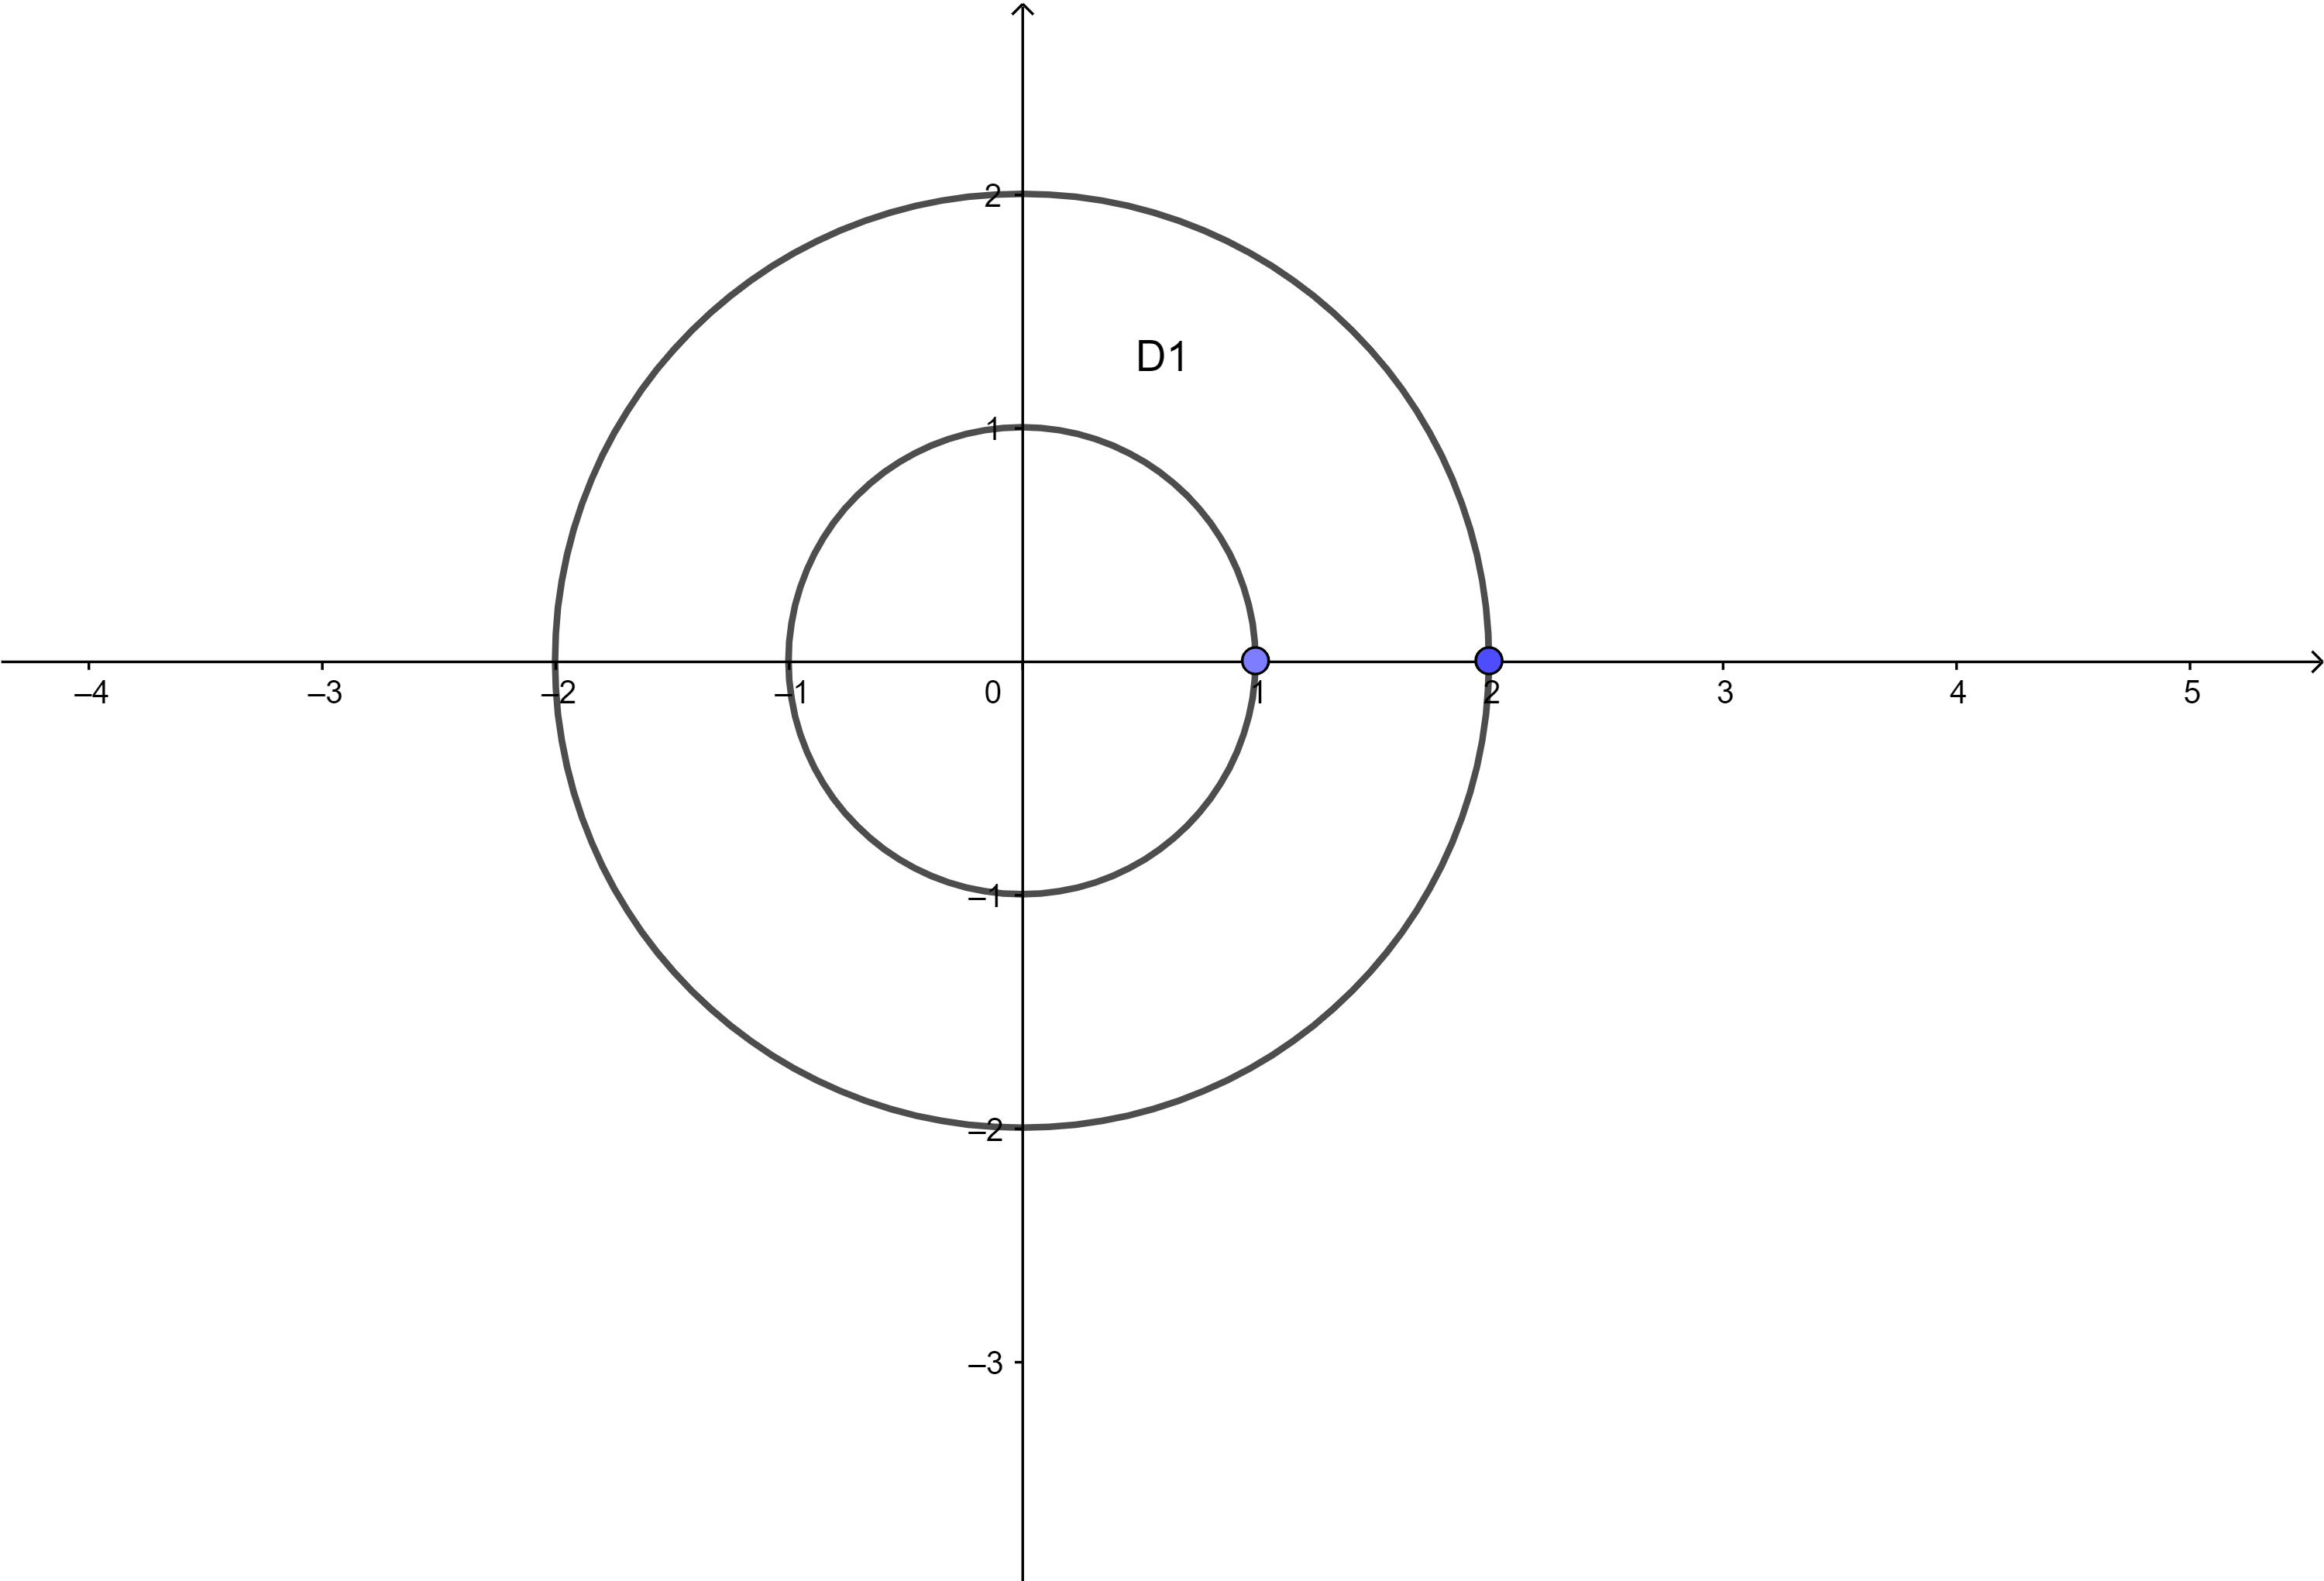
\includegraphics[scale = 0.8]{lec34_2} 
		\end{center}
	
		Разлагая функцию $ f(z) $ на простые имеем:
		
		\[ f(z) = \frac{1}{3(1 + z)} + \frac{1}{3(z - 2)} = \frac{1}{3z(1 + \frac{1}{z})} - \frac{1}{3(1 - \frac{z}{2})} = \left[ |\frac{1}{z}| < 1,\, |\frac{z}{2}| < 1 \right] = \]
		
		\[ = \frac{1}{3z} \sum\limits_{n = 0}^{\infty} \frac{(-1)^n}{z^n} - \frac{1}{3} \sum\limits_{n = 0}^{\infty} \frac{z^n}{2^n} = \frac{1}{3} \left( -\sum\limits_{n = 0}^{\infty} \frac{z^n}{2^n} + \sum\limits_{n = 0}^{\infty} \frac{(-1)^n}{z^{n + 1}} \right) \]
	\end{enumerate}
\end{exmp}

\end{document}
